\documentclass[12pt]{article}
\input{bayesuvius.sty}
\begin{document}

\begin{figure}[h!]\centering
\begin{minipage}{.4\linewidth}
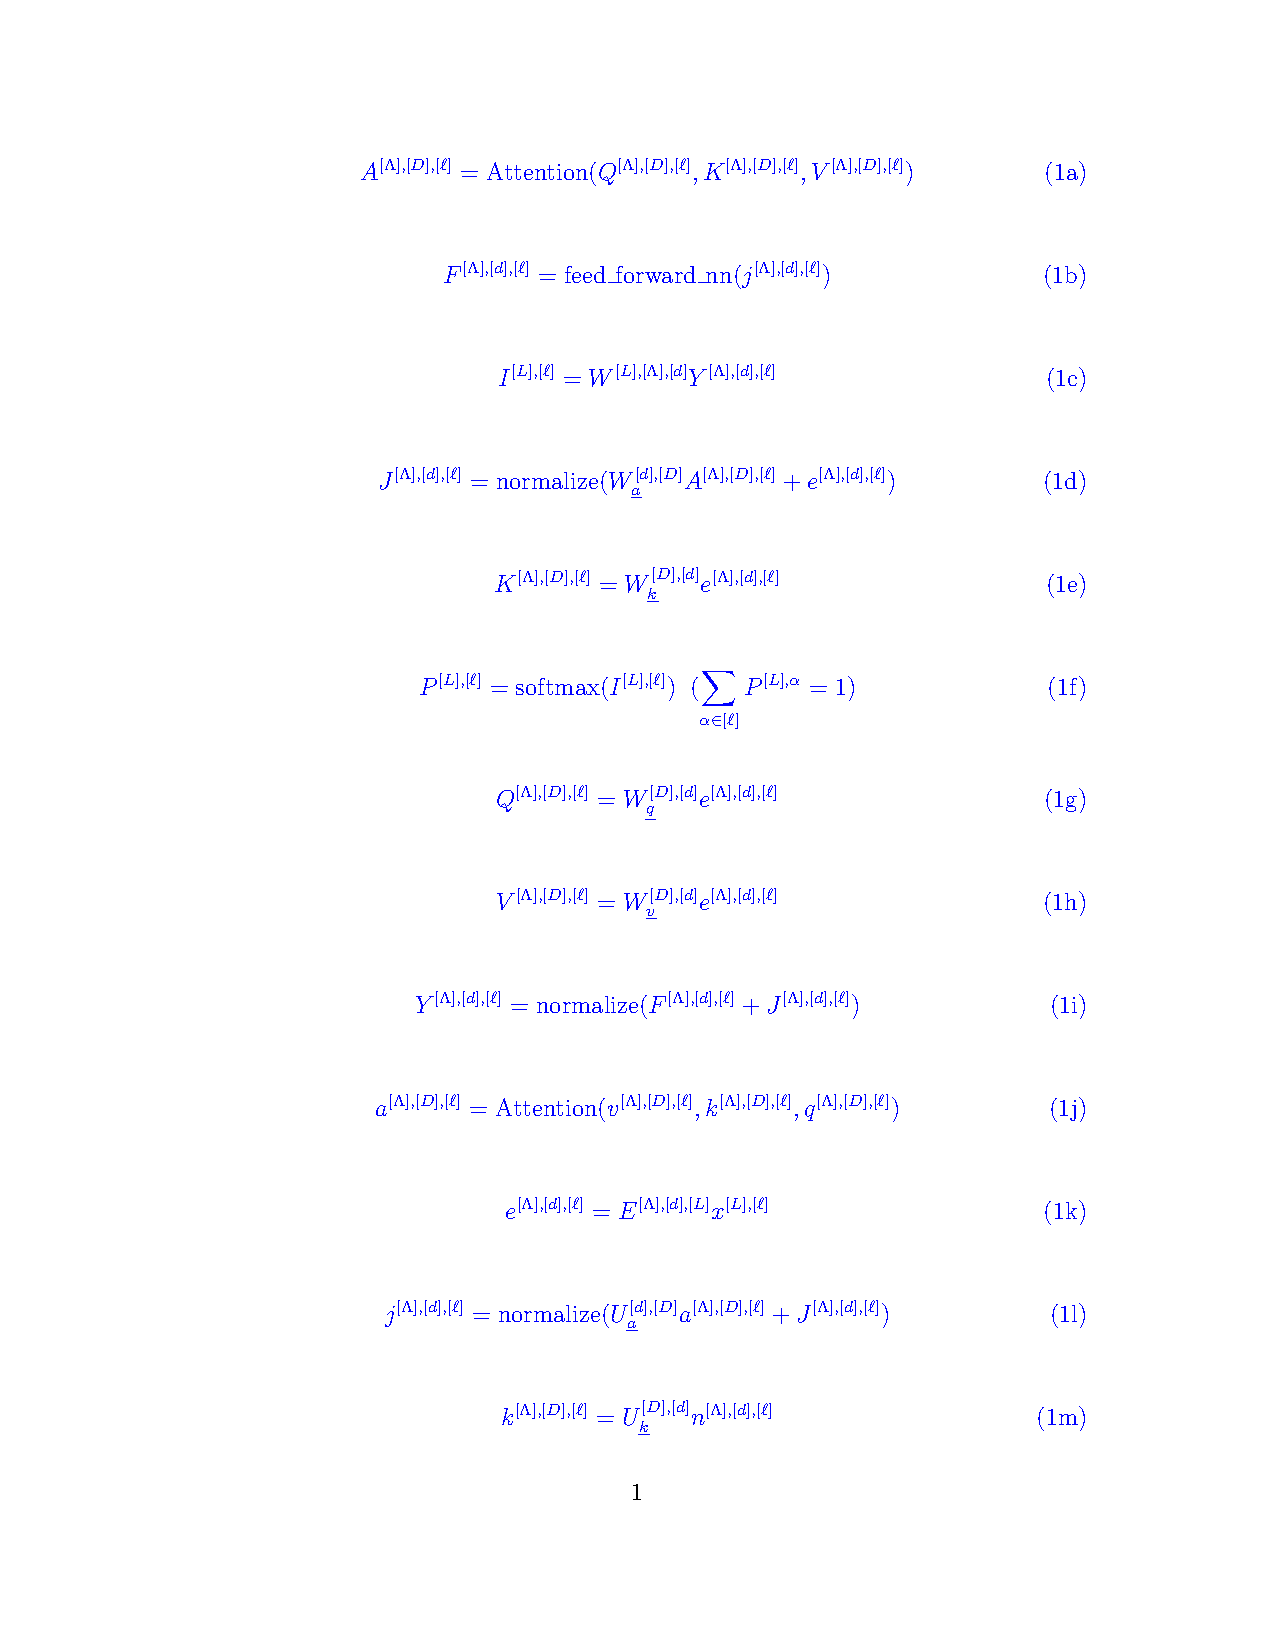
\includegraphics[width=2in]{decoder.jpg}
\end{minipage}%blank lines between minispaces breaks this
\begin{minipage}{.6\linewidth}
$$\xymatrix@R=2.5pc@C=0.2pc{
&&&*+[F*:SpringGreen]{\underline{P}^{[L],[\ell]}}
\\
&&&*+[F*:Orchid]{\underline{I}^{[L],[\ell]}}\ar[u]
\\
&&&*+[F*:yellow]{\underline{Y}^{[\Lambda],[d], [\ell]}}\ar[u]
\\
&&*+[F*:SkyBlue]{\underline{F}^{[\Lambda],[d], [\ell]}}\ar[ur]&
\\
&*+[F*:Dandelion]{\underline{o}^{[\Lambda],[d],[\ell]}}\ar[rr]&&*+[F*:yellow]{\underline{j}^{[\Lambda],[d], [\ell]}}\ar[ul]\ar[uu]
\\
*+[F*:Dandelion]{\underline{v}^{[\Lambda],[D], [\ell]}}\ar[ur]&*+[F*:Dandelion]{\underline{k}^{[\Lambda],[D], [\ell]}}\ar[u]&*+[F*:Dandelion]{\underline{q}^{[\Lambda],[D], [\ell]}}\ar[ul]&
\\
*+[F*:yellow]{\underline{n}^{[\Lambda],[d], [\ell]}}\ar[ur]\ar[u]&&&*+[F*:yellow]{\underline{a}^{[\Lambda],[d], [\ell]}}\ar[uu]\ar[ul]
\\
&*+[F*:Dandelion]{\underline{O}^{[\Lambda],[d],[\ell]}}\ar[urr]&&
\\
*+[F*:Dandelion]{\underline{Q}^{[\Lambda],[D], [\ell]}}\ar[ur]&*+[F*:Dandelion]{\underline{K}^{[\Lambda],[D], [\ell]}}\ar[u]&*+[F*:Dandelion]{\underline{V}^{[\Lambda],[D], [\ell]}}\ar[ul]&
\\
&&&*+[F*:gray]{\underline{e}^{[\Lambda],[d],[\ell]}}\ar[ull]\ar[ulll]\ar[ul]\ar[uuu]
\\
&&&*+[F*:Lavender]{\underline{x}^{[L],[\ell]}}\ar[u]
\save
\POS"3,1"."10,1"."3,4"."10,4"!C*+<4.0em>\frm{-,}
\restore
\\
*+[F-,]{\;\;}&\text{$\Lambda$ layers}
}$$
\end{minipage}
\caption{Decoder.}
\label{fig-texnn-for-decoder}
\end{figure}

\begin{subequations}

\begin{equation}\color{blue}
F^{[\Lambda],[d], [\ell]} = \text{feed\_forward\_nn}(j^{[\Lambda],[d], [\ell]})
\label{eq-B-fun-decoder}
\end{equation}

\begin{equation}\color{blue}
I^{[L],[\ell]} = W^{[L],[\Lambda], [d]}Y^{[\Lambda],[d], [\ell]}
\label{eq-I-fun-decoder}
\end{equation}

\begin{equation}\color{blue}
K^{[\Lambda],[D], [\ell]} = W_\rvk^{[D],[d]}e^{[\Lambda],[d],[\ell]}
\label{eq-K-fun-decoder}
\end{equation}

\begin{equation}\color{blue}
O^{[\Lambda],[d],[\ell]} = \text{multi\_head\_attention}(Q^{[\Lambda],[D], [\ell]},K^{[\Lambda],[D], [\ell]},V^{[\Lambda],[D], [\ell]})
\label{eq-o-fun-decoder}
\end{equation}

\begin{equation}\color{blue}
P^{[L],[\ell]} = \text{softmax}(I^{[L],[\ell]})\;\;\text{$(\sum_{\alp\in[\ell]}P^{[L], \alp}=1)$}
\label{eq-G-fun-decoder}
\end{equation}

\begin{equation}\color{blue}
Q^{[\Lambda],[D], [\ell]} = W_\rvq^{[D],[d]}e^{[\Lambda],[d],[\ell]}
\label{eq-Q-fun-decoder}
\end{equation}

\begin{equation}\color{blue}
V^{[\Lambda],[D], [\ell]} = W_\rvv^{[D],[d]}e^{[\Lambda],[d],[\ell]}
\label{eq-V-fun-decoder}
\end{equation}

\begin{equation}\color{blue}
Y^{[\Lambda],[d], [\ell]} = \text{normalize}(F^{[\Lambda],[d], [\ell]} + a^{[\Lambda],[d], [\ell]})
\label{eq-Y-fun-decoder}
\end{equation}

\begin{equation}\color{blue}
a^{[\Lambda],[d], [\ell]} = \text{normalize}(O^{[\Lambda],[d],[\ell]} + e^{[\Lambda],[d],[\ell]})
\label{eq-a-fun-decoder}
\end{equation}

\begin{equation}\color{blue}
e^{[\Lambda],[d],[\ell]} = E^{[\Lambda],[d],[L]}x^{[L],[\ell]}
\label{eq-p-fun-decoder}
\end{equation}

\begin{equation}\color{blue}
j^{[\Lambda],[d], [\ell]} = \text{normalize}(o^{[\Lambda],[d],[\ell]} + a^{[\Lambda],[d], [\ell]})
\label{eq-j-fun-decoder}
\end{equation}

\begin{equation}\color{blue}
k^{[\Lambda],[D], [\ell]} = U_\rvk^{[D],[d]}n^{[\Lambda],[d], [\ell]}
\label{eq-k-fun-decoder}
\end{equation}

\begin{equation}\color{blue}
n^{[\Lambda],[d], [\ell]} = \;\;\text{Prior comming from Encoder.}
\label{eq-n-fun-decoder}
\end{equation}

\begin{equation}\color{blue}
o^{[\Lambda],[d],[\ell]} = \text{multi\_head\_attention}(v^{[\Lambda],[D], [\ell]},k^{[\Lambda],[D], [\ell]},q^{[\Lambda],[D], [\ell]})
\label{eq-O-fun-decoder}
\end{equation}

\begin{equation}\color{blue}
q^{[\Lambda],[D], [\ell]} = U_\rvq^{[D],[d]}a^{[\Lambda],[d], [\ell]}
\label{eq-q-fun-decoder}
\end{equation}

\begin{equation}\color{blue}
v^{[\Lambda],[D], [\ell]} = U_\rvv^{[D], [d]}n^{[\Lambda],[d], [\ell]}
\label{eq-v-fun-decoder}
\end{equation}

\begin{equation}\color{blue}
x^{[L],[\ell]} = \;\;\text{prior}
\label{eq-R-fun-decoder}
\end{equation}

\end{subequations}


\end{document}  
